\section{Dominant-set clustering}
A very important limitation of the clustering algorithms we've seen so far (especially the \textbf{partition-based} one) is that they're not able to separate the structure of the data from the clutter: this happens because they're goal is to locate distinct coherent clusters, but they do not work very well in presence of noise.

\imageb{img/dominant_init}{0.55}

Indeed, in certain real-world problems, natural groupings are found among only on a small subset of the data, while the rest of the data shows little or no clustering tendencies. In such situations, it is often \textbf{more important} to \textbf{cluster a small subset} of the data very well, \textbf{rather} than \textbf{optimizing} a \textbf{clustering criterion} over \textbf{all the data points}, particularly in application scenarios where a large amount of noisy data is encountered.

Moreover, while partitional approaches impose that each element cannot belong to more than one cluster, this new approach allows to also consider nodes belonging to two different clusters, hence considering the hypothesis of \textbf{overlapping clusters}.

\imageb{img/dominant_overlapping}{0.7}

\subsection{Graph-theoretic definition of a cluster}
Data to be clustered are represented as an undirected weighted graph with no self-loops: $G=(V, E, \omega)$, where $V=\{1,\dots,n\}$ is the vertex set, $E\subseteq V\times V$ is the edges set and $w: E\rightarrow \mathbb{R}^*_+$ is the positive weight function. Vertices represent data points, edges neighborhood relationships and edge-weights similarity relations. $G$ is then represented with an adjacency matrix $A$, such that $a_{ij} = \omega(i,j)$. Since there are not self-loops we have that $\omega(i,i) = 0$ (main diagonal equal to $0$). From now on, if not otherwise stated, $A$ will represent such matrix. \\
There is \textbf{not} an \textbf{unique} and well defined \textbf{definition} of \textbf{cluster}, but the available literature agrees in two conditions that a cluster should satisfy:
\begin{itemize}
  \item \textbf{High internal homogeneity}, also named \textit{internal criterion}. It means that all the objects inside a cluster should be highly similar to (or have low distance from) each other;
  \item \textbf{High external inhomogeneity}, also named \textit{external criterion}. It means that objects coming from different clusters have low similarity (or high distance).
\end{itemize}
The idea of these criterion is that \textbf{clusters} are groups of objects which are \textbf{strongly similar} to each other if they belong to the same cluster, otherwise they are \textbf{highly dissimilar}. 

\paragraph{Basic definitions.}

Let $S\subseteq V$ be a nonempty subset of vertices and $i \in S$. The \textbf{average weighted degree} of $i$ w.r.t. $S$ is defined as:
\begin{equation}
  \text{awdeg}_S(i)=\frac{1}{|S|}\sum_{j\in S}a_{ij}
\end{equation}
, i.e. it represents the \textbf{average similarity} between entity $i$ and the rest of the entities in $S$. It can be observed that $\text{awdeg}_{\{i\}}(i) = 0$  $\forall i \in V$, since we have no self-loops.\\

\image{img/awdeg.png}{Average weighted degree.}{0.25}

We now introduce a new quantity $\phi$ such that if $j \notin S$:
\begin{equation}
  \phi_S(i, j)=a_{ij}-\text{awdeg}_S(i)
\end{equation}

Intuitively, $\phi_S(i, j)$ measures the \textbf{relative similarity} between $i$ and $j$ with respect to the \textbf{average similarity} between $i$ and its neighbors in $S$. This measures can be either positive or negative.

Let $S\subseteq V$ be a nonempty subset of vertices and $i \in S$. The \textbf{weight} of $i$ w.r.t. $S$ is:
\begin{equation}
  w_S(i)= \begin{cases}
      1 & \text{if } |S| = 1 \text{  (singleton)}\\
      \sum\limits_{j\in S\setminus \{i\}}\phi_{S\setminus \{i\}}(j, i)w_{S\setminus \{i\}}(j) & \text{otherwise}
  \end{cases}
\end{equation}

Furthermore, the \textbf{total weight} of $S$ is defined to be $W(S)=\sum_{i\in S}w_S(i)$.
\image{img/ws.png}{Weight of i w.r.t. the elements in S.}{0.18}
Note that $w_{\{i, j\}}(i)=w_{\{i, j\}}(j)=a_{ij}$ $\forall i, j \in V \land i\neq j$. Then, $w_S(i)$ is computed simply as a function of the weights on the edges of the sub-graph induced by $S$.

Intuitively, $w_S(i)$ gives a measure of the \textbf{similarity} between $i$ and $S\setminus \{i\}$ with respect to the \textbf{overall similarity} among the vertices of $S\setminus \{i\}$. In other words, it represents \textbf{how similar (important)} $i$ is \textbf{with respect to the entities} in $S$. An important property of this definition is that it induces a sort of \textbf{natural ranking} among the \textbf{vertices} of the graph. 

\begin{figure}[h!]
		\centering
        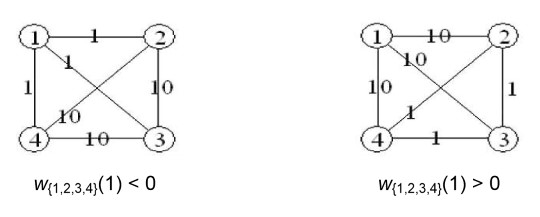
\includegraphics[scale = 1.0]{img/total weight rxample.jpg}
		\label{mi}
        \caption{Examples of total weight}
\end{figure}

As we can see, in the first example we should not add node 1 to the cluster \{1,2,3\}, since it has a low similarity compared with the other nodes (as it can be seen from the value of the total weight), while in the second case we would add node 1 in order to obtain a larger and more coherent cluster.

\paragraph{Dominant set.} A nonempty subset of vertices $S\subset V$ such that $W(T)>0$ for any nonempty $T \subseteq S$, is said to be a \textbf{dominant set} if:
\begin{itemize}
  \item $w_S(i) > 0$, $\forall i \in S \qquad$ (\textit{internal homogeneity})
  \item $w_{S \cup \{i\}}(i) < 0$, $\forall i \notin S \qquad$ (\textit{external homogeneity})
\end{itemize}
These conditions correspond to cluster properties (\textbf{internal homogeneity} and \textbf{external in-homogeneity}). Informally we can say that the \textbf{first condition} requires that \textbf{all the nodes} in the clusters are \textbf{important} for it. The \textbf{second} one assumes that if we consider a \textbf{new point} in the cluster, the \textbf{cluster cohesiveness will be lower}, meaning that the current cluster should be already maximal.\\
By definition, dominant sets are expected to capture \textbf{compact structure}s. Moreover, this definition is equivalent to the one of maximal clique problem when applied to unweighted graphs.

\image{img/dominant_def}{The set of vertices \{1,2,3\} is dominant.}{0.2}

\subsection{Connections of dominant sets}
Dominant sets have intriguing connections with:

\begin{itemize}
    \item \textbf{Game theory}, and concepts like Nash equilibria;
    \item \textbf{Optimization theory}, in particular they are local maximizers of (continuous) quadratic problems;
    \item \textbf{Graph theory} and \textbf{maximal cliques};
    \item \textbf{Dynamical systems theory}.
\end{itemize}

\subsubsection{Game theory}
Game theory is the study of \textbf{mathematical models} of strategic interaction between rational decision-makers. In this sense we can model a new \textbf{clustering game} with the following properties:
\begin{itemize}
	\item \textbf{Symmetric game}, the payoffs for playing a particular strategy depend only on the other strategies employed, not on who is playing them;
	\item \textbf{Complete knowledge}, payoffs, strategies and types of players are known;
	\item Pre-existing set of \textbf{pure strategies}. Players do not behave “rationally” but act according to a pre-programmed behavioral pattern (pure strategy).
\end{itemize}
Data points $V$ are the pure strategies available to the players and the similarity matrix $A$ represents the \textbf{payoff matrix}, which resumes the revenues that each player obtains when a pair of strategies is played. The values $A_{ij}$ and $A_{ji}$ are the revenues obtained by player 1 and player 2 considering that they have player strategies $(i,j) \in V\times V$.
A \textbf{mixed strategy} $x=(x_1, \dots, x_n)^T \in \Delta$ is a probability distribution over the set of pure strategies, which models a stochastic playing strategy of a player. If player 1 and 2 play mixed strategies $(x_1, x_2) \in \Delta \times \Delta$, then the expected payoffs for the players are: $\mathbf{x_1^TAx_2}$ and $\mathbf{x_2^TAx_1}$ respectively.
The goal of the two players of course is to maximize their resulting revenue as much as possible. During the game each player extracts an object $(i,j)$ and the resulting revenue is associated
according to the payoff matrix $A$. Since we are considering $A$ as equal to the similarity matrix, we can say that in order to \textbf{maximize} their revenues the two players should \textbf{coordinate} their strategies so that the \textbf{extracted objects belong to the same cluster}. In other words, only by selecting objects belonging to the same cluster, each player is able to maximize his expected payoff. The unique difference is that the similarity between two equal entities is $0$, meaning that $A_{ii} = 0$. The desired condition is that the two players reach a \textbf{symmetric Nash equilibrium}, a state in which the two players agree about the cluster membership. A \textbf{Nash equilibrium} is a mixed-strategy profile $(x_1,x_2)\in \Delta\times \Delta$ such that no player can improve the expected payoff by changing his playing strategy, given the opponent's strategy being fixed. In other words, it is a \textbf{configuration of strategies} for which \textbf{no player} will deviate from it for its convenience since there is \textbf{no incentive} to change choice. This concept can be expressed with the following expression:
$$y_1^TAx_2 \leq x_1^TAx_2 \qquad y_2^TAx_1 \leq x_2^TAx_1 \qquad \forall (y_1,y_2) \in (V\times V).$$ 
A Nash equilibrium is \textbf{symmetric} if $x_1 = x_2$, meaning that considering a symmetric Nash equilibrium $x \in \Delta$ the two conditions hold in a unique one:
$$y^TAx \leq x^TAx$$

This condition satisfies the \textbf{internal homogeneity} criterion required by the dominant set definition, but it does \textbf{not} include any kind of constraint that guarantees the \textbf{maximality condition}. In order to satisfy this condition it is necessary to look for a different type of Nash Equilibrium, known as \textbf{Evolutionary Stable Strategy (ESS)}. 

\paragraph{ESS.} A symmetric Nash equilibrium $x\in \Delta$ is an \textbf{evolutionary stable strategy} (ESS) if it satisfies also:
$$y^TAx = x^TAx \implies x^TAy > y^TAy \qquad \forall y \in \Delta\setminus\{x\}$$

$$y^TAx = x^TAx \implies x^TAy < x^TAx \qquad \forall y \in \Delta\setminus\{x\}$$
Even if the strategy $y$ provides the same payoff of the strategy $x$, it is better to play $x$ since the payoff against itself is greater than the one provided by $y$. The two strategies $x$ and $y$ represents two Nash Equilibrium, but only $x$ is an ESS.\\
In conclusion we can say that the \textbf{ESSs of the clustering game} with affinity matrix $A$ are in \textbf{correspondence} with \textbf{dominant sets} of the same clustering problem instance. However, we can also conclude that \textbf{ESSs} are in \textbf{one-to-one} correspondence to \textbf{(strict) local solutions of StQPs} (Standard Quadratic optimization Problems).\\
It is possible to say that ESSs abstract well the main characteristic of a cluster:
\begin{itemize}
	\item \textbf{Internal coherency:} High mutual support of all elements within the group.
	\item \textbf{External incoherency:} Low support from elements of the group to elements outside the group.
\end{itemize}

\subsubsection{Optimization theory}
\textbf{Clusters} are commonly represented as $n$-dimensional \textbf{vectors} expressing the participation of each node to a cluster. Large numbers denote a strong participation, while zero values no participation. The \textbf{cohesiveness} of a cluster can be computed using:
\begin{equation}
f(x)=x^\top Ax
\end{equation}
where $A$ is the \textbf{symmetric} real-valued matrix with null diagonal. \textbf{Clustering} can now be formulated as the problem of \textbf{finding the vector} $x$ that \textbf{maximizes} $f$. The objective function has to be \textbf{normalized}. For this aim simplex constraints are imposed. This yields the following \textbf{standard quadratic optimization problem} whose \textbf{local solution} corresponds to a \textbf{maximally cohesive cluster}:
\begin{equation}\label{SPQ}
\begin{array}{lcl}
\text{max} & x^TAx \\
\text{s.t.} & x \in \Delta
\end{array}
\end{equation}
where
\begin{equation}
\Delta=\{x\in\mathbb{R}^n:x\geq 0 \land x^\top x = 1\}
\end{equation}
is the \textbf{standard simplex} of $\mathbb{R}^n$.\\

\image{img/standardSimplex.png}{Standard simplex on $\mathbb{R}^3$.}{0.35}

As we can see, this problem is quite similar to the one presented in the previous Chapter, but the difference relies in the constraint.

In conclusion \textbf{dominant sets} can be put in \textbf{one-to-one correspondence} (modulo a technical condition) with \textbf{strict local maximizers} of a \textbf{quadratic function over the simplex}. As opposed to many other clustering algorithms, which try to find the global optimum of some energy function, dominant sets can be found by mining local solutions.

\subsubsection{Graph theory and maximal cliques}
Suppose we have a \textbf{binary similarity matrix} and an unweighted undirected graph $G = (V,E)$, then:

\begin{itemize}
    \item A \textbf{clique} is a subset of mutually adjacent vertices;
    \item A \textbf{maximal clique} is a clique that is not contained in a larger one;
\end{itemize}

It was proved that \textbf{EES's} are in \textbf{one-to-one correspondence} to \textbf{maximal cliques} of $G$. 

\subsection{Finding dominant sets}
One of the major \textbf{advantages} of using \textbf{dominant sets} is that the procedure that allows to find them can be written with few lines of code. There are several dominant set clustering approaches:
\begin{itemize}
	\item To get a \textbf{single} dominant set cluster use \textbf{replicator dynamics};
	\item To get a \textbf{partition} use a simple \textit{peel-off} strategy: iteratively find a dominant set and remove it from the graph, until all vertices have been clustered;
	\item To get \textbf{overlapping clusters}, enumerate dominant sets. 
\end{itemize}
The \textbf{replicator dynamics} (RD) are \textbf{deterministic game dynamics} that have been developed in evolutionary game theory. They consider an idealized scenario whereby individuals are repeatedly drawn at random from a large, ideally infinite, population to play a two-player game. In contrast to classical game theory, here players are not supposed to behave rationally or to have complete knowledge of the details of the game. They act instead according to an inherited behavioral pattern, or pure strategy, and it is supposed that some evolutionary selection process operates over time on the distribution of behaviors.\\
Let $x_i(t)$ be the population share playing pure strategy $i$ at time $t$. The state of the population at time $t$ is: $x(t) = (x_1(t),\dots,x_n(t))\in\Delta$.\\
We define an evolution equation, derived from Darwin's principle of nature selection:
$$\dot{x_i} = x_i~g_i(x)$$
where $g_i$ specifies the rate at which pure strategy $i$ replicates.
$$\frac{\dot{x_i}}{x_i} \propto \text{payoff of pure strategy }i\text{ - average population payoff}$$
which yields:
$$\dot{x_i} = x_i[(Ax)_i - x^TAx]$$
where $(Ax)_i$ is the $i$-th component of the vector and $x^TAx$ is the average payoff for the population. If we have a result which is better than the average strategy, then there is an improvement.
We can see $\dot{x_i}$ as the fraction of the total number of players that's using strategy $i$. As $\dot{x_i}$ increases, so does the number of players using it; conversely, if $\dot{x_i}$ decreases, the strategy will likely disappear.  

\paragraph{Theorem.} A point $x\in\Delta$ is a Nash equilibrium if and only if $x$ is the limit point of a replicator dynamics trajectory starting from the interior of $\Delta$.
Furthermore, if $x\in\Delta$ is an ESS, then it is an asymptotically stable equilibrium point for the replicator dynamics.\\

Assuming that the payoff matrix $A$ is symmetric $(A = A^T)$, we call this type of game as a doubly symmetric game. Thanks to this assumption we can derive some conclusions:
\begin{itemize}
	\item (\textbf{\textit{Fundamental Theorem of Natural Selection}}.) For any doubly symmetric game, the average population payoff $f(x) = x^TAx$ is strictly increasing along any non-constant trajectory of replicator dynamics, meaning that $\frac{df(x(t))}{dt} \geq 0$ $\forall t \geq0$, with equality if and only if $x(t)$ is a stationary point.
	\item (\textit{\textbf{Characterization of ESSs}}.) For any doubly symmetric game with payoff matrix $A$, the following statements are equivalent:
	\begin{itemize}
		\item $x\in \Delta^{ESS}$
		\item $x \in \Delta$ is a strict local maximizer of $f(x) = x^TAx$ over the standard simplex $\Delta$.
		\item $x\in\Delta$ is asymptotically stable in the replicator dynamics.
	\end{itemize}
\end{itemize}


A well-known \textbf{discretization} of replicator dynamics, which assumes non-overlapping generations, is the following (assuming a non-negative $A$): 
$$
x_i(t+1) = x_i(t)\frac{A(x(t))_i}{x(t)^TAx(t)}
$$
which inherits most of the dynamical properties of its continuous-time counterpart. The idea here is the same as above: we are evolving dominant strategies. Since $A(x(t))_i$ is the payoff for strategy $i$ and $x(t)^\top Ax(t)$ is the average payoff, if the ratio is greater than 1 then the strategy is dominant and the derivative is positive increasing.
\image{img/rep_dynamics}{MATLAB implementation of discrete-time replicator dynamics}{0.4}
The components of the \textbf{converged vector} give us a measure of the \textbf{participation} of the corresponding vertices in the cluster, while the \textbf{value} of the \textbf{objective function} measures the \textbf{cohesiveness} of the cluster.

\subsection{Image segmentation}
An image is represented as an edge-weighted undirected graph, where \textbf{vertices} correspond to \textbf{individuals pixels} and edge-weights reflect the \textbf{similarity} between pairs of vertices. The \textbf{clustering} problem consists on extracting \textbf{dominant sets} from an input image, below is proposed the pseudo-code version of the solution with dominant sets:

\image{img/dominantSetAlg.png}{Pseudo-code for image segmentation.}{0.5}
Remember that to find a single dominant set we used replicator dynamics.


\subsection{Properties}
\begin{itemize}
	\item \textbf{Well separation between structure and noise.} In such situations it is often more important to cluster a small subset of the data very well, rather than optimizing a clustering criterion over all the data points, particularly in application scenarios where a large amount of noisy data is encountered;
	
	\item \textbf{Overlapping clustering}. In some cases we can have that two distinct clusters share some points, but partitional approaches impose that each element cannot be long to more than one cluster;
	
	\item Dominant sets can be found by mining \textbf{local solutions}, so it is not necessary to look for global solutions;
	
	\item Performs very well in presence of \textbf{noise} and \textbf{outliers};
		
	\item Makes \textbf{no assumptions} on the \textbf{structure} of the \textbf{affinity matrix}, being it able to work with asymmetric and even negative similarity functions;
	
	\item Does \textbf{not} require a \textbf{priori knowledge} on the \textbf{number of clusters} (since it extracts them sequentially).
	
	\item Leaves \textbf{clutter} elements \textbf{unassigned} (useful, e.g., in figure/ground separation or one-class clustering problems);
	
	\item Generalizes naturally to \textbf{hypergraph clustering problems};

        \item It allows to rank cluster's elements according to their \textbf{centrality}.
\end{itemize}
